\documentclass{school-22.211-notes}
\date{February 22, 2012}

\begin{document}
\maketitle

\topic{Wide Resonance Approximations}
The wide resonance approximation is: 
\begin{align}
\RI_{\eff} &= \int \sigma_r(u) \frac{\sigma_d}{\sigma_r(u) + \sigma_d} \du \\
&= \ln \left(\frac{E_2}{E_1} \right) \frac{ \int \sigma_r(E) \frac{\sigma_d}{\sigma_r(E) + \sigma_d} \frac{1}{E} \dE}{ \int \frac{\sigma_d}{\sigma_r(E) + \sigma_d} \frac{1}{E} \dE}
\end{align}
Notice wide resonance approximation $\RI_{\eff}$ only depends on cross sections: $\sigma_d$ is assumed to be based on material composition of the reactor, and $\sigma_r(E)$ are from libraries. There is no need for flux spectrum. 

The wide resonance approximation says that we ignore scattering of U238 because its width is large compared with the approximately 1\% energy it can lose upon scattering. To improve this approximation, sometimes people use the potential scattering of 11.39 barns. 

Wide resonance approximations match direct MC results near infinite dilution. 

\topic{Narrow Resonance Approximations}
Narrow resonance approximations assume the opposite of the wide resonance approximation, that the neutron is going to be out of the resonance upon one scattering. This approximation is good for higher energy. For instance, at 100 keV, scattering lose 1 keV, which is larger than the 25 eV spacing of \ce{^{238}U}. 

However, the results on the slides come out to be that narrow resonance approximation is not really any better than the wide resonance approximation at higher energy, so there must be some other physics going on. 


\topic{Narrow vs. Wide Resonance Approximations}
Wide resonance approximation agrees pretty well with MC results without U238 scattering; narrow resonance approximation agrees alright with the MC results with U238 scattering. Notice adding in scattering would change the low dilution factor results. See Figure~\ref{wide-vs-narrow}.

Compare with MC results using real U238 and U235 xs data, the real results fall between the wide and the narrow approximations for the high dilution factor; but for the low dilution factor, that is, when there are lots of resonance material (uranium), the physics gets complicated: 
\begin{itemize}
\item Non 1/E slowing down sources;
\item Non constant moderator xs;
\item Resonance scattering alters sources;
\item We may have multiple resonance in each RI group; that is, each of our RI does not include a single resonance anymore;
\item Resonance interference between \ce{^{235}U} and \ce{^{238}U}; eg: \ce{^{238}U}'s resonance spacing is 25 eV, whereas \ce{^{235}U}'s resonance spacing is 5 eV, that is, for each \ce{^{238}U} resonance, there are multiple \ce{^{235}U} resonances on top of it. 
\end{itemize}

\begin{figure}
  \centering
  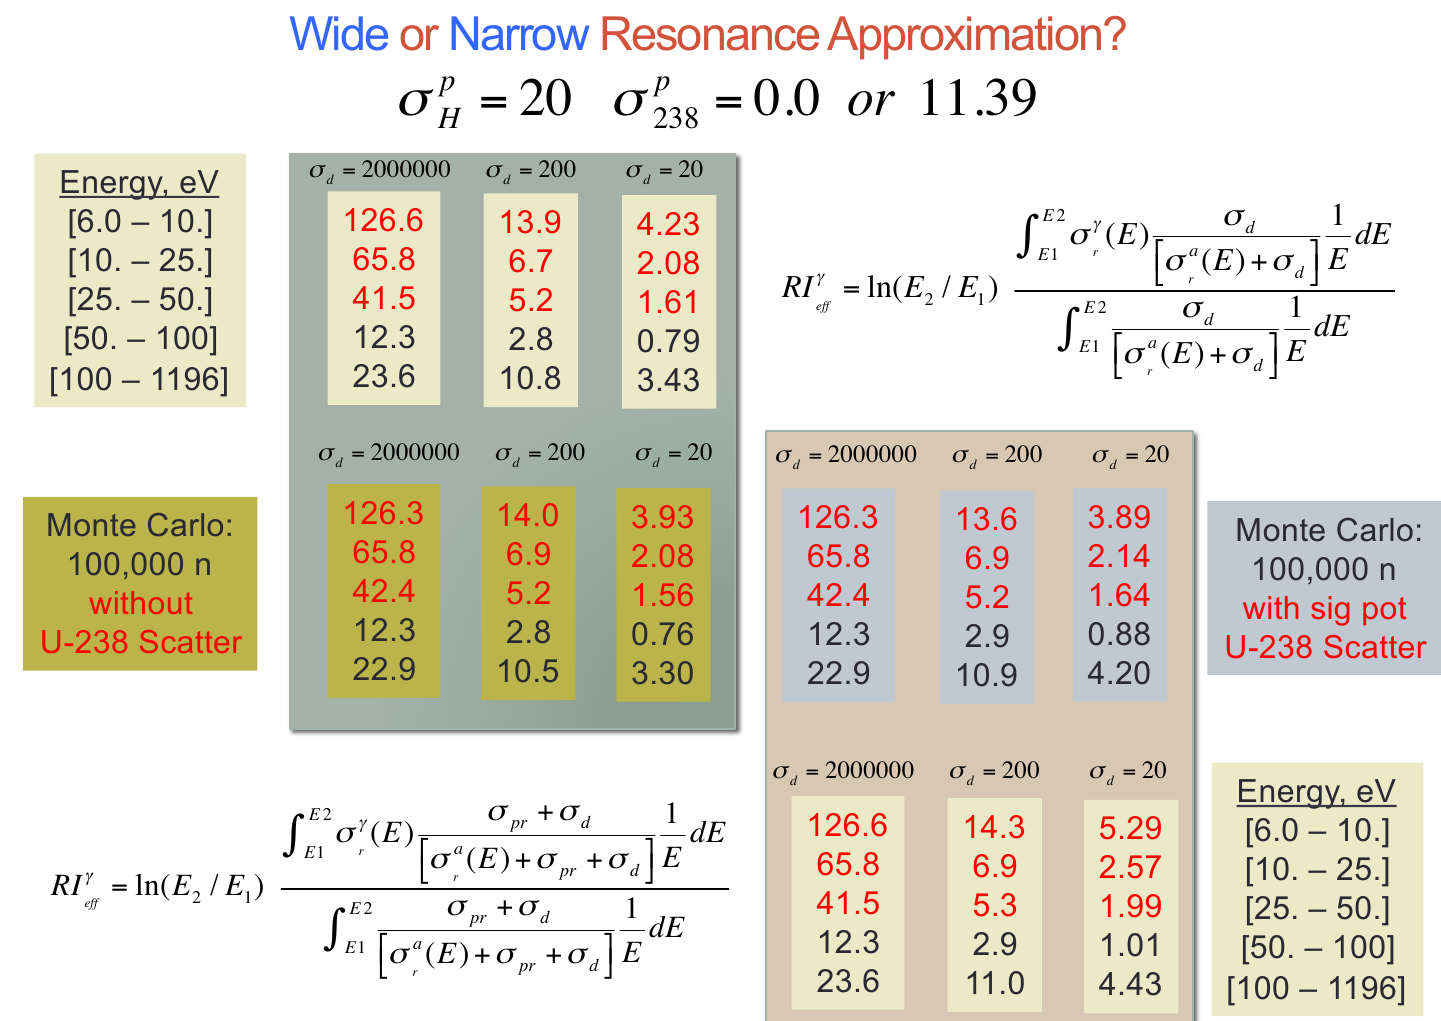
\includegraphics[width=4in]{images/narrow-vs-wide-resonance.png}
  \caption{Comparison Of Wide and Narrow Resonance Approximation} \label{wide-vs-narrow}
\end{figure}



\topic{NJOY Modeling of Resonance Parameters}
The normal procedure for generating multi-group xs in a code like NJOY includes:
\begin{enumerate}
\item use code to Doppler broaden cross sections for each resonance isotope for range of temperatures (eg, 300, 600, 900, 2000K); 
\item use code to apply the narrow or wide resonance models for a range of dilution xs (eg, 20000, 2000, 200, 20 barns); 
\item edit RIs or multi-group xs for your desired energy structure; 
\item build tables of xs vs. dilution xs and temperature;
\item for downstream computations, interpolate for the dilution cross section and temperature of each material in the simulation to obtain accurate multigroup cross sections for that specific applications. 
\end{enumerate}
Note that tables are general and do not have to be computed. 

A better procedure for generating multi-group cross sections includes:
\begin{enumerate}
\item the same;
\item use code to solve real neutron slowing down problem for a range of dilution cross sections (eg, 20000, 2000, 200, 20 barns);
\item consider including a mix of resonance absorbers to make the spectrum as appropriate to the desired application as possible;
\item the same;
\item the same;
\item the same.
\end{enumerate}

For downstream applications that require cross section data, for each resonance group,
\begin{enumerate}
\item For each composition, evaluate the material temperature and isotopic densities. 
\item Evaluate Dancoff from pin diameter, lattice pitch, etc. 
\item Compute the escape cross section for each resonance absorber.
\item Evaluate group cross section (or RI) using Dancoff, potential and escape cross sections by interpolating cross section (or RI) tables at appropriate temperatures. 
\end{enumerate}
The point is, for real application, it is rarely possible to just use someone else's cross section table; we almost certainly need to generate xs suitable for our application. 


\end{document}
